% nleguide.tex
% v1.0, released 31 Jan 2019
% Copyright 2019 Cambridge University Press

\documentclass{nle}

\usepackage{amsmath}
\usepackage{graphicx}
\usepackage{natbib}

\begin{document}
\label{firstpage}

\lefttitle{\LaTeX\ Supplement}
\righttitle{Natural Language Engineering}

\papertitle{Article}

\jnlPage{1}{00}
\jnlDoiYr{2019}
\doival{10.1017/xxxxx}

\title{Natural Language Engineering: \LaTeX\footnote{To know more information about LaTeX and its packages, try https://ctan.org/?lang=en} Guidelines for~authors}

\begin{authgrp}
\author{Cambridge Author}
\affiliation{Electronic Products and Composition Group,\\
        Printing Division, Cambridge University Press, CB2 2BS\\
        \email{texline@cambridge.org}}
\end{authgrp}

\history{(Received xx xxx xxx; revised xx xxx xxx; accepted xx xxx xxx)}
%\received{20 March 1995; revised 30 September 1998}

\begin{abstract}
This guide is for authors who are preparing papers for the {\em Natural Language Engineering} journal using the \LaTeX\ document preparation
system and the CUP NLE style file.
\end{abstract}

\maketitle

\section{Introduction}

The layout design for the {\em Natural Language Engineering} journal
has been implemented as a \LaTeX\ style file. The NLE style file is based
on the ARTICLE style as discussed in the \LaTeX\ manual. Commands which
differ from the standard \LaTeX\ interface, or which are provided in addition
to the standard interface, are explained in this guide. This guide is not a
substitute for the \LaTeX\ manual itself.

\subsection{Introduction to \LaTeX}

The \LaTeX\ document preparation system is a special version of the
\TeX\ typesetting program. \LaTeX\ adds to \TeX\ a collection of
commands which simplify typesetting by allowing the author to
concentrate on the logical structure of the document rather than
its visual layout.

\LaTeX\ provides a consistent and comprehensive document preparation
interface. There are simple-to-use commands for generating a table of
contents, lists of figures and/or tables, and indexes. \LaTeX\ can
automatically number list entries, equations, figures, tables, and
footnotes, as well as parts, chapters, sections and subsections.
Using this numbering system, bibliographic citations, page references
and cross references to any other numbered entity ({\it e.g.\ } chapter,
section, equation, figure, list entry) are quite straightforward.

\subsection{The NLE document class}

The use of document class allows a simple change of style (or style option)
to transform the appearance of your document. The CUP NLE class file preserves
the standard \LaTeX\ interface such that any document which can be produced
using the standard \LaTeX\ ARTICLE style can also be produced with the
NLE style. However, the fonts (sizes) and measure of text is slightly different
from that for ARTICLE, therefore line breaks will change and it is possible
that equations may need re-setting.

\section{Additional facilities}

In addition to all the standard \LaTeX\ design elements, the NLE style
includes the following feature:
\begin{itemize}
  \item Extended commands for specifying a short version
        of the title and author(s) for the running
        headlines.
\end{itemize}
Once you have used this additional facility in your document,
do not process it with a standard \LaTeX\ style file.

\subsection{Titles authors' names and affiliation}

In the NLE style, the title of the article and the author's name (or authors'
names) are used both at the beginning of the article for the main title and
throughout the article as running headlines at the top of every page.
The title is used on odd-numbered pages (rectos) and the author's name appears
on even-numbered pages (versos).
Although the main heading can run to several lines of text, the running head
line must be a single line.

Moreover, the main heading can also incorporate new line commands
({\it e.g.\ } \verb"\\") but these are not acceptable in a running headline.
To enable you to specify an alternative short title and author's name, the
standard \verb"\righttitle" and \verb"\lefttitle" commands have been used to print the running headline. If more authors has to be used in \verb"\author" command then each authors should be captured in separate \verb"\author" command.
\verb"\affiliation" command is used to call the affiliation, if more affiliations has to be used in \verb"\affiliation" command then each affiliations should be captured in separate \verb"\affiliation" command.
\verb"\email" command should be used inside the affiliation as shown below.
%
\begin{verbatim}
\lefttitle{\LaTeX\ Supplement}
\righttitle{Natural Language Engineering}
  \title{The full title which can be as long
   as necessary}
\begin{authgrp}
  \author{Author's name}
  \affiliation{the affiliation if necessary
  \email{email}}
\end{authgrp}
\end{verbatim}
%

\subsection{Abstract}

The NLE style provides for an abstract which is produced by the following
commands
%
\begin{verbatim}
  \begin{abstract}  ...  \end{abstract}
\end{verbatim}

\subsection{Lists}

The NLE style provides the three standard list environments.
\begin{itemize}
  \item Bulleted lists, created using the \verb"itemize" environment.
  \item Numbered lists, created using the \verb"enumerate" environment.
  \item Labelled lists, created using the \verb"description" environment.
\end{itemize}

\subsection{Footnotes}

The NLE journal style uses superior numbers for footnote
references.\footnote{This shows how a footnote is typeset.}

\section{Some guidelines for using standard facilities}

The following notes may help you achieve the best effects with the NLE style
file.

\subsection{Sections}

\LaTeX\ provides five levels of section headings and they are all
defined in the NLE style file:
\begin{itemize}
  \item \verb"\section".
  \item \verb"\subsection".
  \item \verb"\subsubsection".
  \item \verb"\paragraph".
  \item \verb"\subparagraph".
\end{itemize}
Section numbers are given for sections, subsection and subsubsection headings.

\subsection{Running headlines}

As described above, the title of the article and the author's name (or authors'
names) are used as running headlines at the top of every page.
The title is used on odd-numbered pages (rectos) and the author's name appears
on even-numbered pages (versos).

The \verb"\pagestyle" and \verb"\thispagestyle" commands should {\em not\/} be
used.
Similarly, the commands \verb"\markright" and \verb"\markboth" should not be
necessary.


\subsection{Tables}

The {\tt figure} and {\tt table} environments are implemented as described in
the \LaTeX\ Manual to
provide consecutively numbered floating inserts for illustrations and tables
respectively.
The standard inserts and their captions are formatted centred.
Line breaks in captions can be inserted as required using \verb"\\".

The NLE style file will cope with most positioning of your tables
and you should not normally use the optional positional qualifiers on the
\verb"table" environment which would override these decisions.
Normal journal style sets the table caption first, followed by a double
rule, the table body and a double rule at the bottom.  Single rules and
spanner rules (\verb"\cline") can be used to separate headings from the
columns.  For example, Table~\ref{sample-table} is produced using the
following commands:\par
%
{\fontsize{7}{9}\selectfont
\begin{verbatim}
\begin{table}
  \tbl{\caption{Results of Overloading for 3 Experimental Setups}}
  {\begin{minipage}{25pc}
    \begin{tabular}{@{\extracolsep{\fill}}lcrrrrr}
    \hline
    Program& Expt.&
     CPU\footnote{Seconds of elapsed time on an unloaded Sun 3/50.}&
     RelCPU\footnote{CPU Time relative to experiment (a).}&
     GC& Mem\footnote{Bytes of heap used over the duration of the program.}&
     RelMem\footnote{Memory usage relative to experient (a).}\\
    \hline
    8 Queens& (a)&   2 88&  1 00&    6&   1 7M&  1 00\\\hdashline
    &         (b)&  32 51& 11 29&  193&  48 9M& 28 76\\\hdashline
    &         (c)&   7 90&  2 74&   42&  11 3M&  6 65\\\hdashline
    Primes&   (a)&   4 89&  1 00&   19&   5 3M&  1 00\\\hdashline
    &         (b)&  47 54&  9 72&  204&  54 5M& 10 28\\\hdashline
    &         (c)&  10 08&  2 06&   47&  13 0M&  2 45\\\hdashline
    Nfib&     (a)&  21 65&  1 00&  161&  40 4M&  1 00\\\hdashline
    &         (b)& 221 65& 10 24& 1382& 349 0M&  8 64\\\hdashline
    &         (c)&  21 30&  0 98&  161&  42 0M&  1 03\\\hdashline
    KWIC&     (a)&   7 07&  1 00&   15&   6 3M&  1 00\\\hdashline
    &         (b)&  34 55&  4 89&  109&  47 8M&  7 59\\\hdashline
    &         (c)&  31 62&  4 47&   53&  45 0M&  7 14\\\hdashline
    \hline
    \end{tabular}
    \vspace{-2\baselineskip}
  \end{minipage}}
  \label{sample-table}
\end{table}
\end{verbatim}}
%
\noindent Notice the use of the \verb"" macro to obtain the centered
decimal points, inside the body of the table.

\begin{table}[h!]
  \tbl{\caption{Results of Overloading for 3 Experimental Setups}}
 {\begin{minipage}{25pc}
    \begin{tabular}{@{\extracolsep{\fill}}lcrrrrr}
    \hline
    Program& Expt.&
     CPU\footnote{Seconds of elapsed time on an unloaded Sun 3/50.}&
     RelCPU\footnote{CPU Time relative to experiment (a).}&
     GC& Mem\footnote{Bytes of heap used over the duration of the program.}&
     RelMem\footnote{Memory usage relative to experient (a).}\\
    \hline
    8 Queens& (a)&   2 88&  1 00&    6&   1 7M&  1 00\\\hdashline
    &         (b)&  32 51& 11 29&  193&  48 9M& 28 76\\\hdashline
    &         (c)&   7 90&  2 74&   42&  11 3M&  6 65\\\hdashline
    Primes&   (a)&   4 89&  1 00&   19&   5 3M&  1 00\\\hdashline
    &         (b)&  47 54&  9 72&  204&  54 5M& 10 28\\\hdashline
    &         (c)&  10 08&  2 06&   47&  13 0M&  2 45\\\hdashline
    Nfib&     (a)&  21 65&  1 00&  161&  40 4M&  1 00\\\hdashline
    &         (b)& 221 65& 10 24& 1382& 349 0M&  8 64\\\hdashline
    &         (c)&  21 30&  0 98&  161&  42 0M&  1 03\\\hdashline
    KWIC&     (a)&   7 07&  1 00&   15&   6 3M&  1 00\\\hdashline
    &         (b)&  34 55&  4 89&  109&  47 8M&  7 59\\\hdashline
    &         (c)&  31 62&  4 47&   53&  45 0M&  7 14\\
    \hline
    \end{tabular}
  \end{minipage}}
  {\begin{tabnote}
  This is the sample text to show the table notes.
  \end{tabnote}}
  \label{sample-table}
\end{table}

The \verb"tabular" environment should be used to produce ruled tables;
it has been modified for the NLE style in the following ways:
\begin{enumerate}
  \item Additional vertical space is inserted above and below a horizontal rule
        (produced by \verb"\hline");
  \item Tables are centred, and span the full width of the page; that is,
  they are similar to the tables that would be produced by
  \verb"\begin{minipage}" \verb"{\textwidth}".
\end{enumerate}
Because of this reformatting, vertical rules should not be used;
furthermore, commands to
redefine quantities such as \verb"\arraystretch" should be omitted. If
the old tabular facilities are needed, there is a new environment,
\verb"oldtabular", which has none of the reformatting; it should be used
in exactly the same way.

\subsection{Illustrations (or figures)}

The NLE style will cope with most positioning of your illustrations
and you should not normally use the optional positional qualifiers on
the \verb"figure" environment which would override these decisions.
Figure captions should be below the figure itself, therefore the \verb"\caption"
command should appear after the figure or space left for an illustration.

Figure~\ref{sample-figure} shows an example onw working with LaTeX code to load art files. \verb"\includegraphics" commnad is to load art files \verb"scale" option used in \verb"\includegraphics" is to reduce the art. EPS format will be compiled using LaTeX. PNG, PDF and JPG format art files are loaded in the same command but the TeX file should be compiled using PDFLaTeX:
%
\begin{verbatim}
  \begin{figure}
    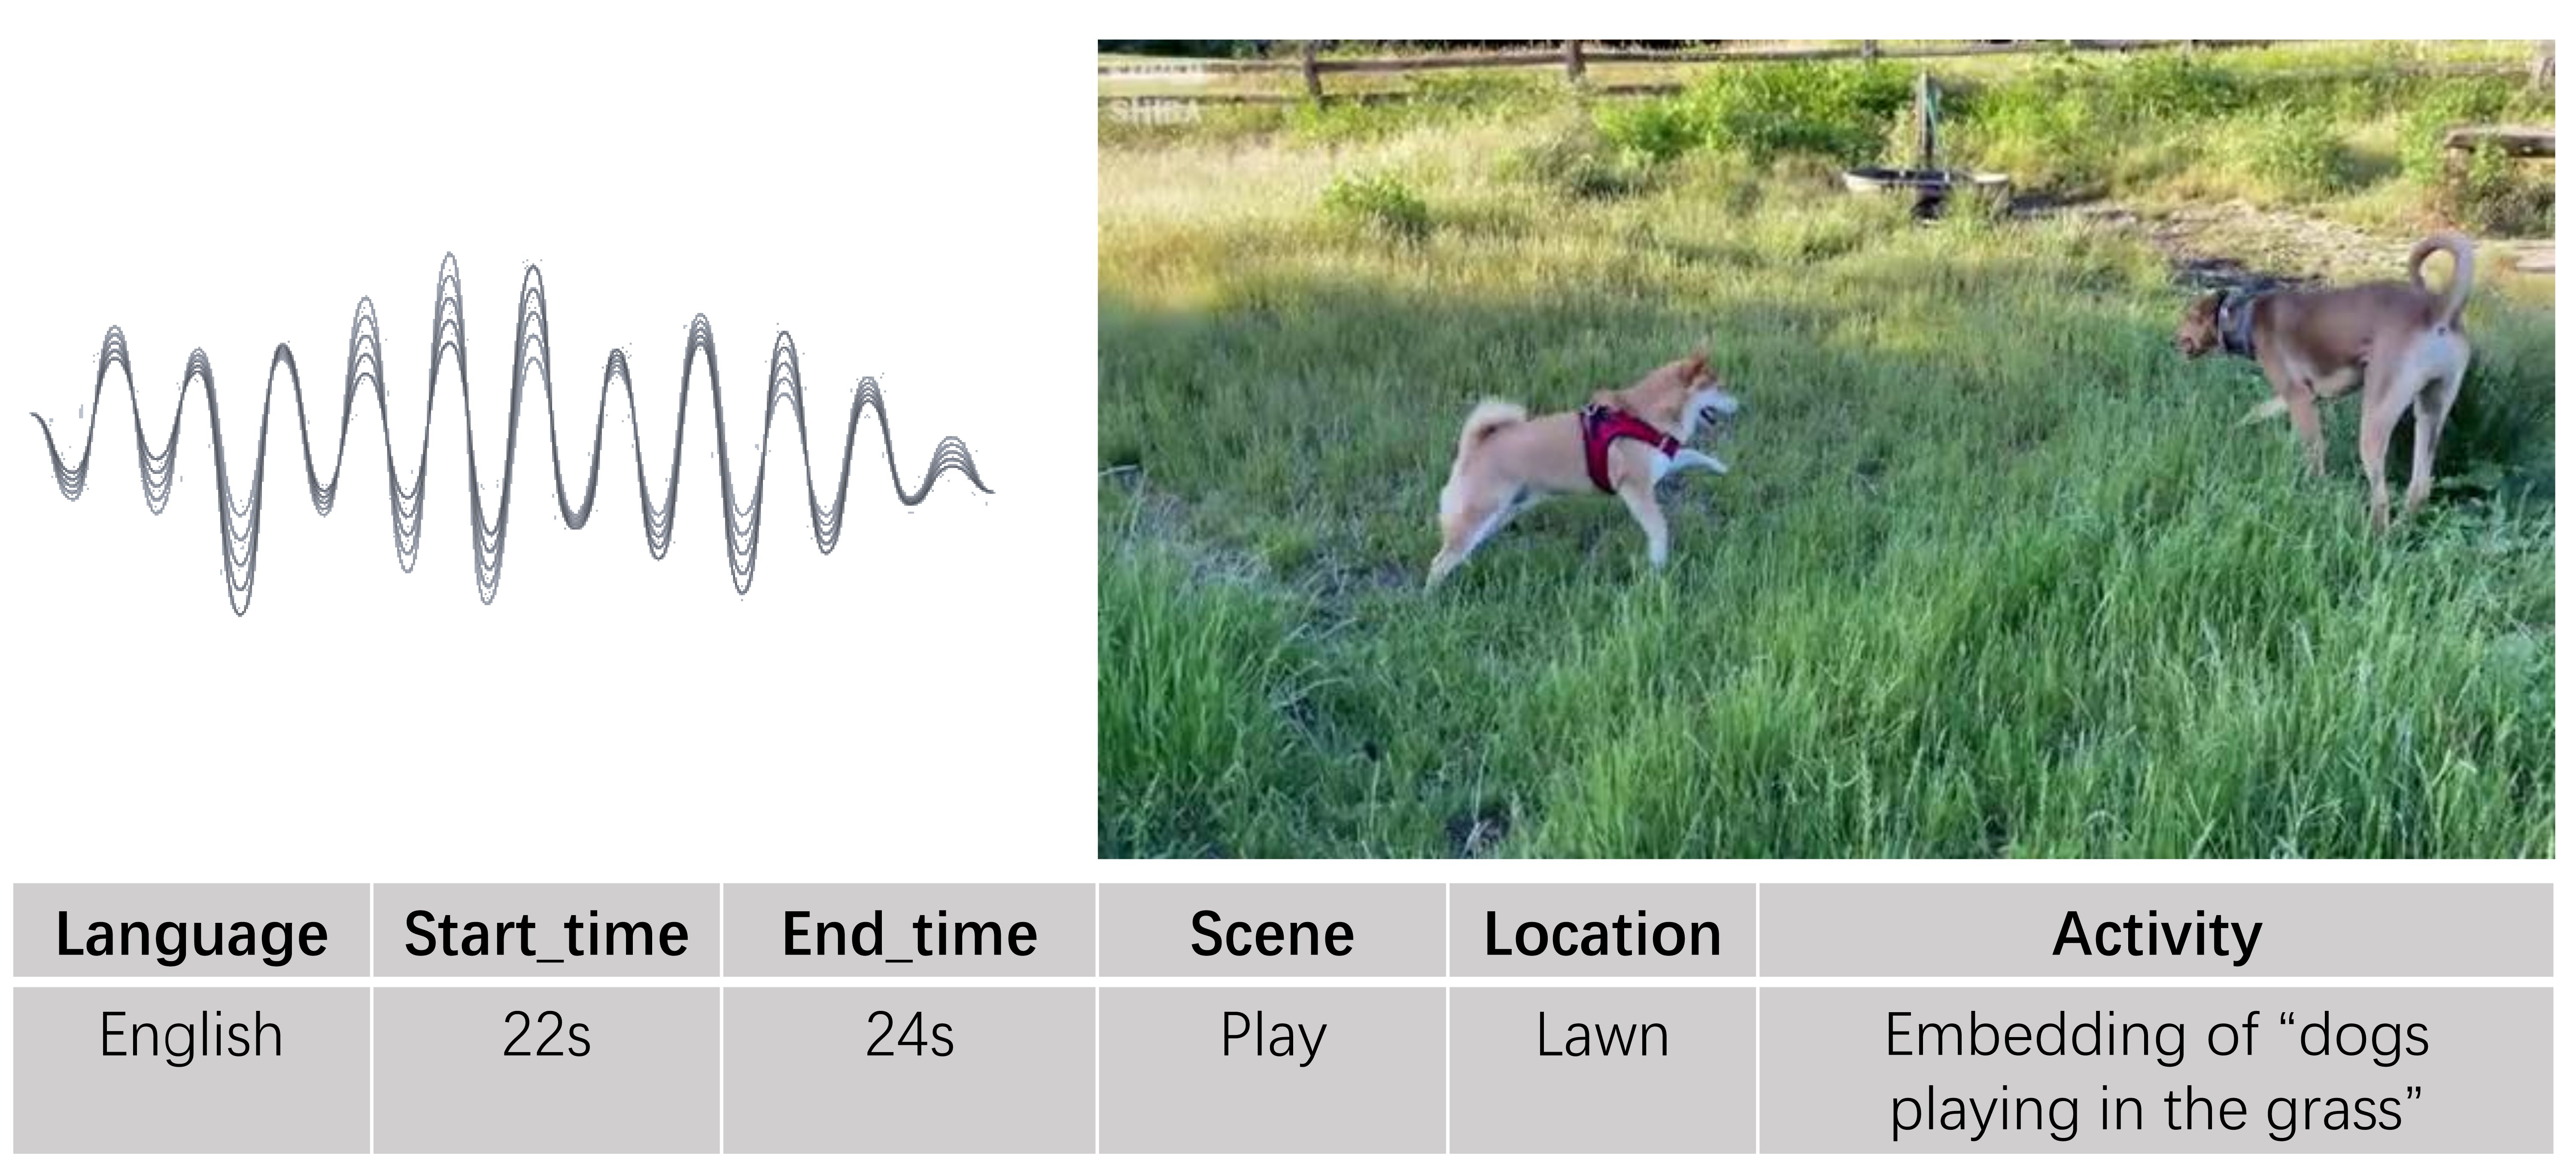
\includegraphics[scale=.4]{sample.eps}
    \caption{An example figure with space for artwork.}
    \label{sample-figure}
  \end{figure}
\end{verbatim}
%
\begin{figure}[t]
  \centerline{\vbox to 8pc{\hbox to 10pc{}}}
  %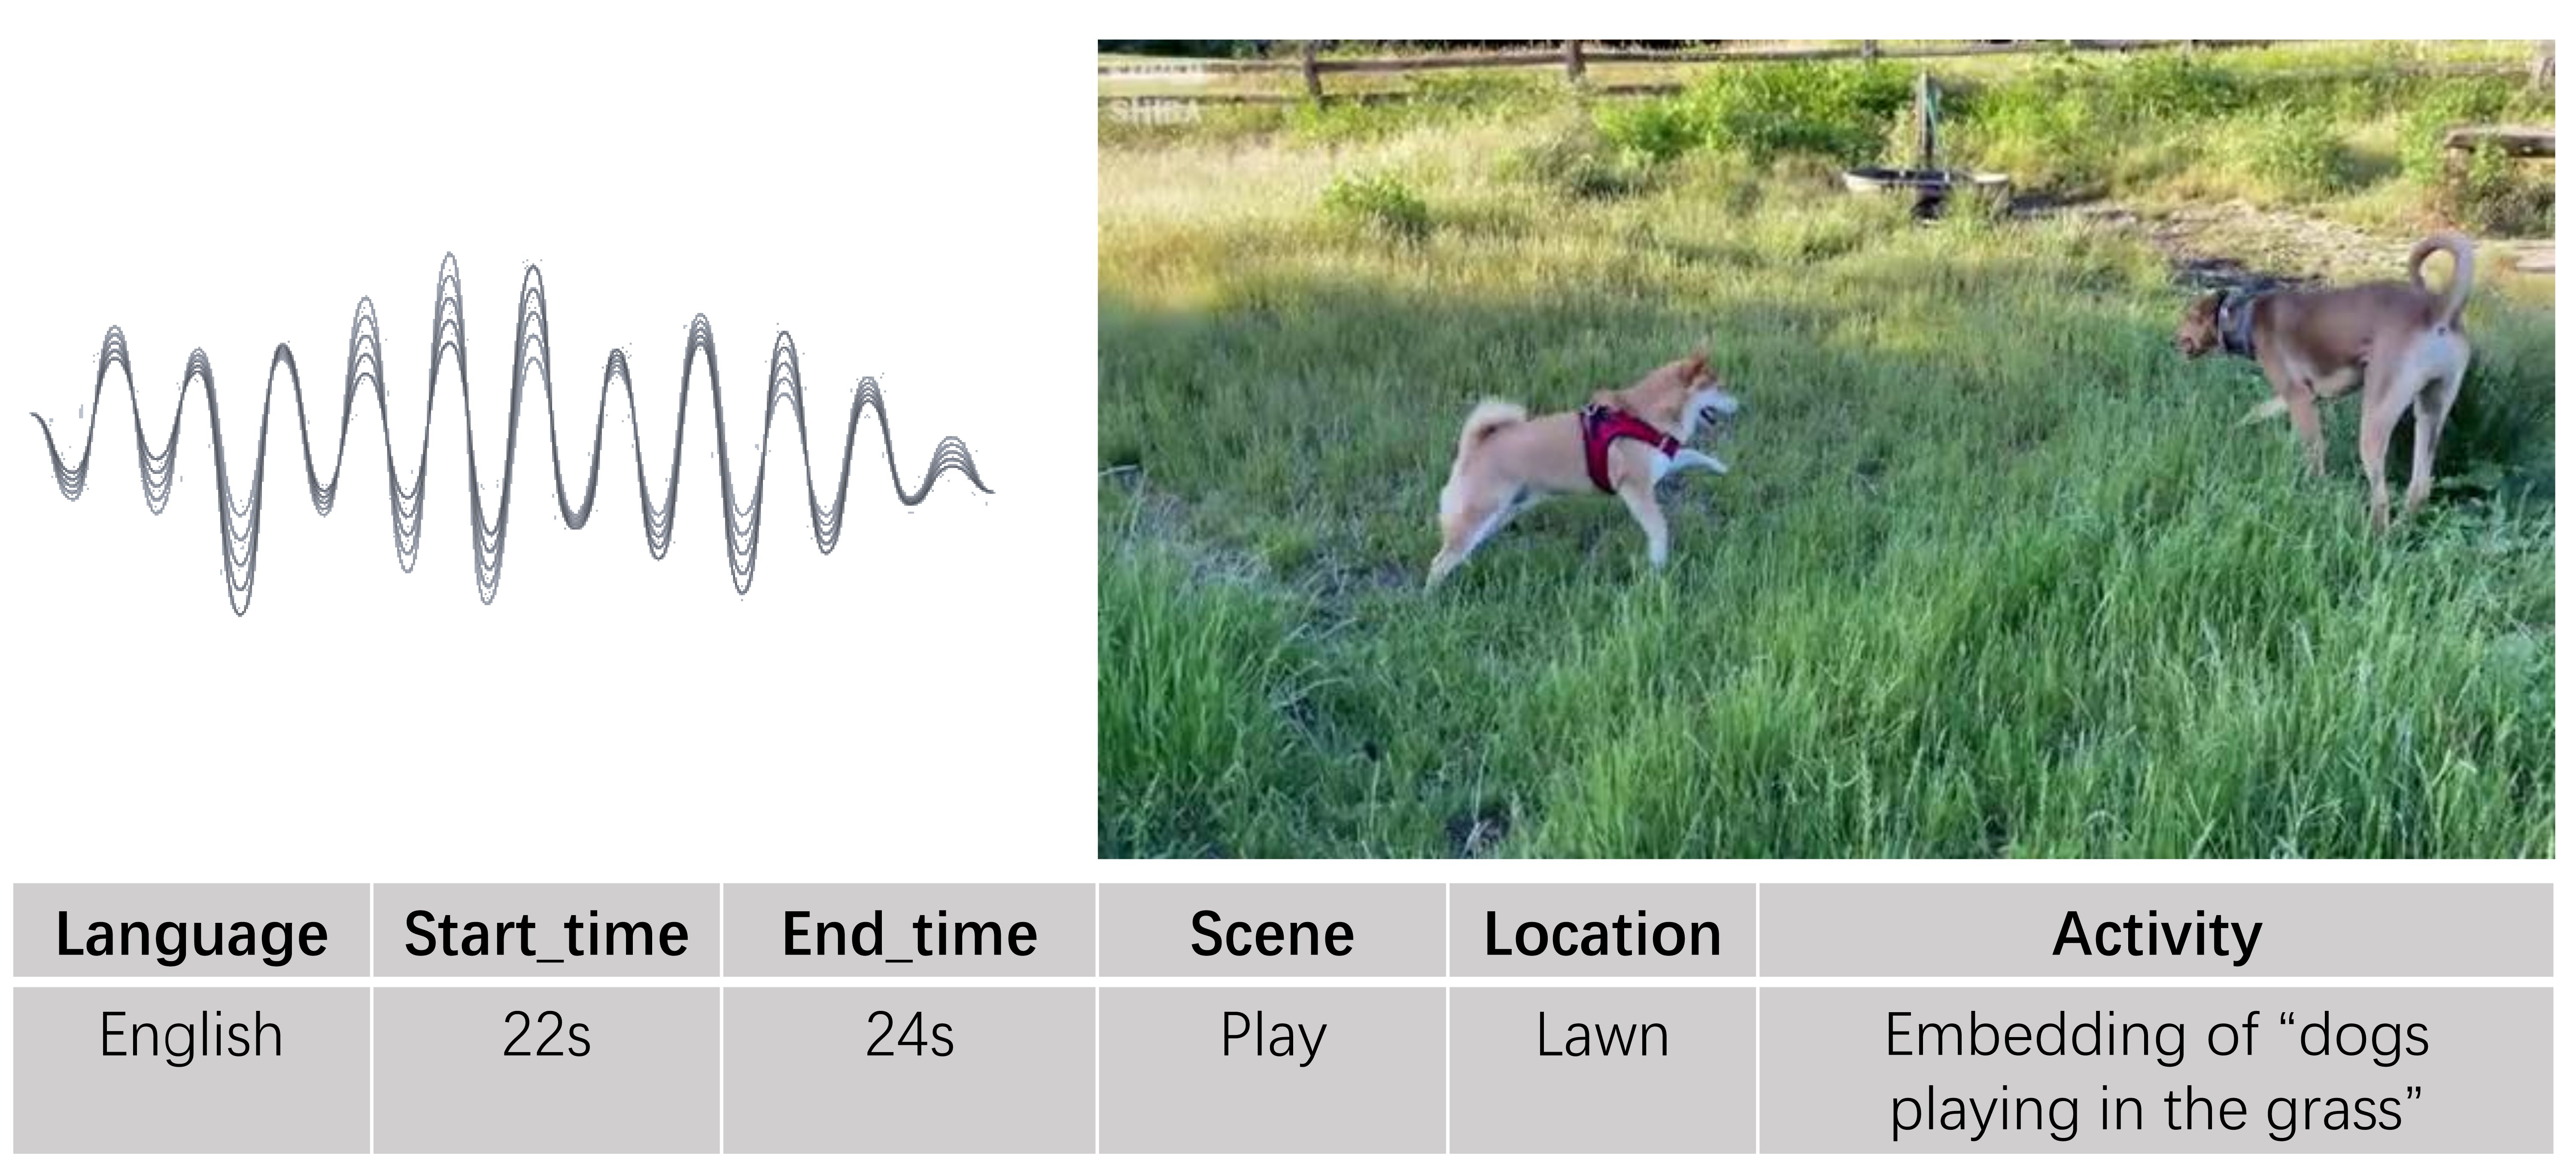
\includegraphics[scale=.4]{sample.eps}
  \caption{An example figure with space for artwork.}
  \label{sample-figure}
\end{figure}
%
The vertical depth should correspond roughly to the artwork you will submit;
it will be adjusted to fit the final artwork exactly.

\subsection{Creating new theorem-like environments}

You can create your own environments in \LaTeX, and although you may already
be familiar with \verb"\newtheorem", you will not have seen the other two
commands explained below.

\verb"\newtheorem" is a standard command used for creating new
        theorem-like environments, such as theorems, corollaries, lemmas,
        conjectures and propositions, with the body of the text
        (automatically) in italic.

\section{Mathematics}

The NLE class file will centre displayed mathematics, and will insert the
correct space above and below if standard \LaTeX\ commands are used; for
example use \verb"\[ ... \]" and \emph{not} \verb"$$ ... $$". Do not leave
blank lines above and below displayed equations unless a new paragraph is
really intended.

\verb"amsmath.sty" is common package to handle various type math equations. The amsmath descriptions are available in the document can be find in the web link \verb"https://ctan.org/pkg/amsmath?lang=en"

\subsection{Numbering of equations}

The \verb"subequations" and \verb"subeqnarray" environments have been
incorporated into the NLE class file (see Section~\ref{sub:amstex} regarding
the \verb"subequations" environment). Using these two environments,
you can number your equations (\ref{a1}), (\ref{a2}) etc. automatically.
For example, you can typeset
  \begin{subequations}
  \begin{equation}
    a_1 \equiv (2\Omega M^2/x)^{\textstyle\frac{1}{4}}
      y^{\textstyle\frac{1}{2}}\label{a1}
  \end{equation}
  and
  \begin{equation}
    a_2 \equiv (x/2\Omega)^{\textstyle\frac{1}{2}}k_y/M.\label{a2}
  \end{equation}
  \end{subequations}
by using the \verb"subequations" environment as follows:
%
\begin{verbatim}
  \begin{subequations}
  \begin{equation}
    a_1 \equiv (2\Omega M^2/x)^{\textstyle\frac{1}{4}}
      y^{\textstyle\frac{1}{2}}\label{a1}
  \end{equation}
  and
  \begin{equation}
    a_2 \equiv (x/2\Omega)^{\textstyle\frac{1}{2}}k_y/M.\label{a2}
  \end{equation}
  \end{subequations}
\end{verbatim}

\subsubsection{The \texttt{subequations} environment and the
  \texttt{AMSTEX} package} \label{sub:amstex}

The \verb"amstex" (and the \verb"amsmath") packages also define a
\verb"subequations" environment.  The environment in \verb"NLE.cls" is used
by default, as the environments in the AMS packages don't produce the correct
style of output.

Note that the \verb"subequations" environment from the \verb"amstex" package
takes an argument -- you should use an `a' to give \verb"\alph" style
subequations. e.g.
\begin{verbatim}
  \begin{subequations}{a}  ...  \end{subequations}
\end{verbatim}

\subsection{Bibliography}

As with standard \LaTeX, there are two ways of producing a bibliography;
either by compiling a list of references by hand (using a
\verb"thebibliography" environment), or by using BibTeX with a suitable
bibliographic database with the bibliography style provided with the nleguide.tex like \verb"\bibliographystyle{nlelike}". The nle.bst will produce the bibliography which is similar to NLE style but not exactly. If any modification has to be made with nle.bst can be adjusted during manuscript preparation but the updated bst file should be given with source files. However, contributors are encouraged to format
their list of references style outlined in section~\ref{fullref}
below.

\subsubsection{References in the text}

References in the text are given by author and date.
Whichever method is used to produce the bibliography, the references in
the text are done in the same way. Each bibliographical entry has a key,
which is assigned by the author and used to refer to that entry in the
text. There is one form of citation -- \verb"\cite{key}" -- to produce the
author and date. Thus, \cite{sal90} is produced~by
\begin{verbatim}
  \cite{sal90}.
\end{verbatim}

\verb"natbib.sty" is common package to handle various reference and its cross citations. The natbib descriptions are available in the document can be find in the web link \verb"https://ctan.org/pkg/natbib?lang=en"

\subsubsection{List of references}\label{fullref}

The following listing shows some references prepared in the style of the
journal.
%
{\fontsize{7}{9}\selectfont
\begin{verbatim}
  \begin{thebibliography}{}
    \bibitem[\protect\citename{Akmajian and Lehrer }1976]{akm76}
     Akmajian, \& Lehrer, A. 1976. NP-like quantifiers and the
     problem of determining the head of an NP. {\it Linguistic
     Analysis\/} {2}, 295--313.
    \bibitem[\protect\citename{Huddleston }1984]{hud84}
     Huddleston, Rodney. 1984. {\it Introduction to the Grammar of
     English}. Cambridge: Cambridge University Press.
    \bibitem[\protect\citename{McCord }1990]{mcc90}
     McCord, Michael C. 1990. Slot grammar: a system for simpler
     construction of practical natural language grammars. In R.
     Studer (ed.), {\it Natural Language and Logic: International
     Scientific Symposium}, pp.~118--45. Lecture Notes in Computer
     Science. Berlin: Springer-Verlag.
    \bibitem[\protect\citename{Salton {\it et al.}\ }1990]{sal90}
     Salton, Gerald, Zhao, Zhongnan \& Buckley, Chris. 1990.
     A simple syntactic approach for the generation of indexing
     phrases. Technical Report 90--1137, Department of Computer
     Science, Cornell University.
  \end{thebibliography}
\end{verbatim}}
%
This list typesets as shown at the end of this guide.
Each entry takes the form
%
\begin{verbatim}
  \bibitem[\protect\citename{Author(s), }Date]{tag}
    Bibliography entry
\end{verbatim}
%
where \verb"Author(s)"\ should be the author names as they are cited in
the text, \verb"Date" is the date to be cited in the text, and \verb"tag"
is the tag that is to be used as an argument for the \verb"\cite{}" command.
\verb"Bibliography entry" should be the
material that is to appear in the bibliography, suitably formatted.  This
rather unwieldy scheme makes up for the lack of an author-date system in
\LaTeX.

\section{Notes for Editors}

This appendix contains additional information which may be useful to
those who are involved with the final production stages of an article.
Authors, who are generally not typesetting the final pages in the
journal's typeface (Monotype Times), do not need this information.

\subsection{Catchline and date commands}

To be placed in the preamble; for example:

\begin{itemize}
  \item \verb"\jnlDoiYr{2019}"
  \item \verb"\doival{10.1017/xxxxx}"
  \item \verb"\jnlPage{1}{8}"
  \item \verb"\history{(Received xx xxx xxx; revised xx xxx xxx; accepted xx xxx xxx)}"
\end{itemize}

\subsection{Editing citations (when the author has used the
  ${\backslash}$cite command)}

In the past when an automatic \verb"\cite" command produced text in the output
which needed to be changed, the argument (in [ ]) from the bibliography entry
was copied to the location of the \verb"\cite" command and then modified.
The \verb"\cite" command would then be removed as part of this process.

In the near future, we will probably have to supply \TeX\ output which will
need to contain `PDF marks' for interactive browsing.  Clearly by removing
the automatic link to the bibliographic entry (referenced by the \verb"\cite"),
we are making extra work for ourselves later on.

To avoid this, the function of the \verb"\cite" command's optional argument
has been changed. For example, the \verb"\cite" command for the
`\verb"mcc90"' entry gives:
\[ \hbox{(McCord 1990)} \]
but you want the following to appear in the text:
\[ \hbox{(McCord 1990, see p.~119)} \]
you would then use:
\[ \hbox{\verb"\cite[(McCord 1990, see p.~119)]{mcc90}"} \]
to obtain the desired result. Notice that you have to supply
the round brackets as well in the optional argument.

\begin{thebibliography}{}
  \bibitem[\protect\citename{Akmajian and Lehrer, }1976]{akm76}
   Akmajian \& Lehrer A. 1976. NP-like quantifiers and the
   problem of determining the head of an NP. {\it Linguistic
   Analysis\/} {2}, 295--313.
  \bibitem[\protect\citename{Huddleston, }1984]{hud84}
   Huddleston, Rodney. 1984. {\it Introduction to the Grammar of
   English}. Cambridge: Cambridge University Press.
  \bibitem[\protect\citename{McCord, }1990]{mcc90}
   McCord, Michael C. 1990. Slot grammar: a system for simpler
   construction of practical natural language grammars. In R.
   Studer (ed.), {\it Natural Language and Logic: International
   Scientific Symposium}, pp.~118--45. Lecture Notes in Computer
   Science. Berlin: Springer-Verlag.
  \bibitem[\protect\citename{Salton {\it et al.}, }1990]{sal90}
   Salton, Gerald, Zhao, Zhongnan \& Buckley, Chris. 1990.
   A simple syntactic approach for the generation of indexing
   phrases. Technical Report 90--1137, Department of Computer
   Science, Cornell University.
\end{thebibliography}

\label{lastpage}

\end{document}
